\documentclass[border=2pt]{standalone}
\usepackage{pgfplots}
\usepackage{pgfplotstable}
\pgfplotsset{compat=1.18}
\usepackage{xcolor}
\definecolor{amber}{HTML}{E69F00}
\definecolor{teal}{HTML}{009E73}
\definecolor{blue}{HTML}{0072B2}
\definecolor{mauve}{HTML}{CC79A7}
\definecolor{grey}{HTML}{999999}
\definecolor{vermilion}{HTML}{D55E00}
\usepackage{times}

\begin{document}

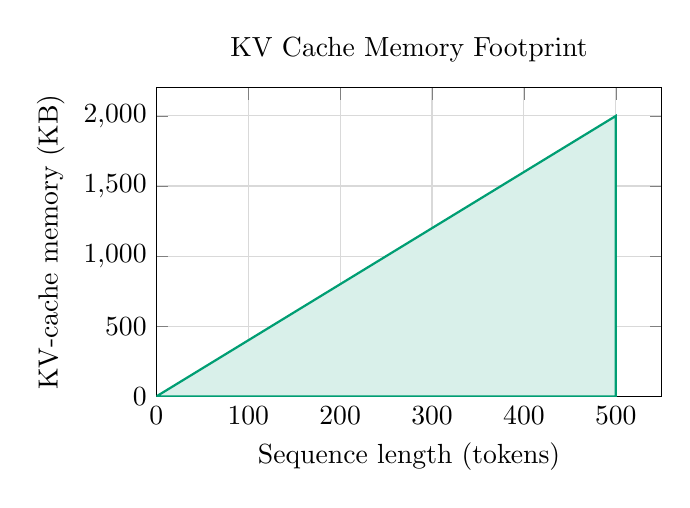
\begin{tikzpicture}
\begin{axis}[
  width=8cm, height=5.5cm,
  xlabel={Sequence length (tokens)},
  ylabel={KV-cache memory (KB)},
  title={KV Cache Memory Footprint},
  grid=major, grid style={gray!30},
  xmin=0, ymin=0,
]
\addplot[color=teal, thick, fill=teal!15] coordinates {(0,0.0000) (50,200.0000) (100,400.0000) (150,600.0000) (200,800.0000) (250,1000.0000) (300,1200.0000) (350,1400.0000) (400,1600.0000) (450,1800.0000) (500,2000.0000)} \closedcycle;
\end{axis}
\end{tikzpicture}
\end{document}
